\section{Additional Figures \& Tables}
\label{sec:additional_figures_tables}


\begin{figure}[h!]
    \centering
    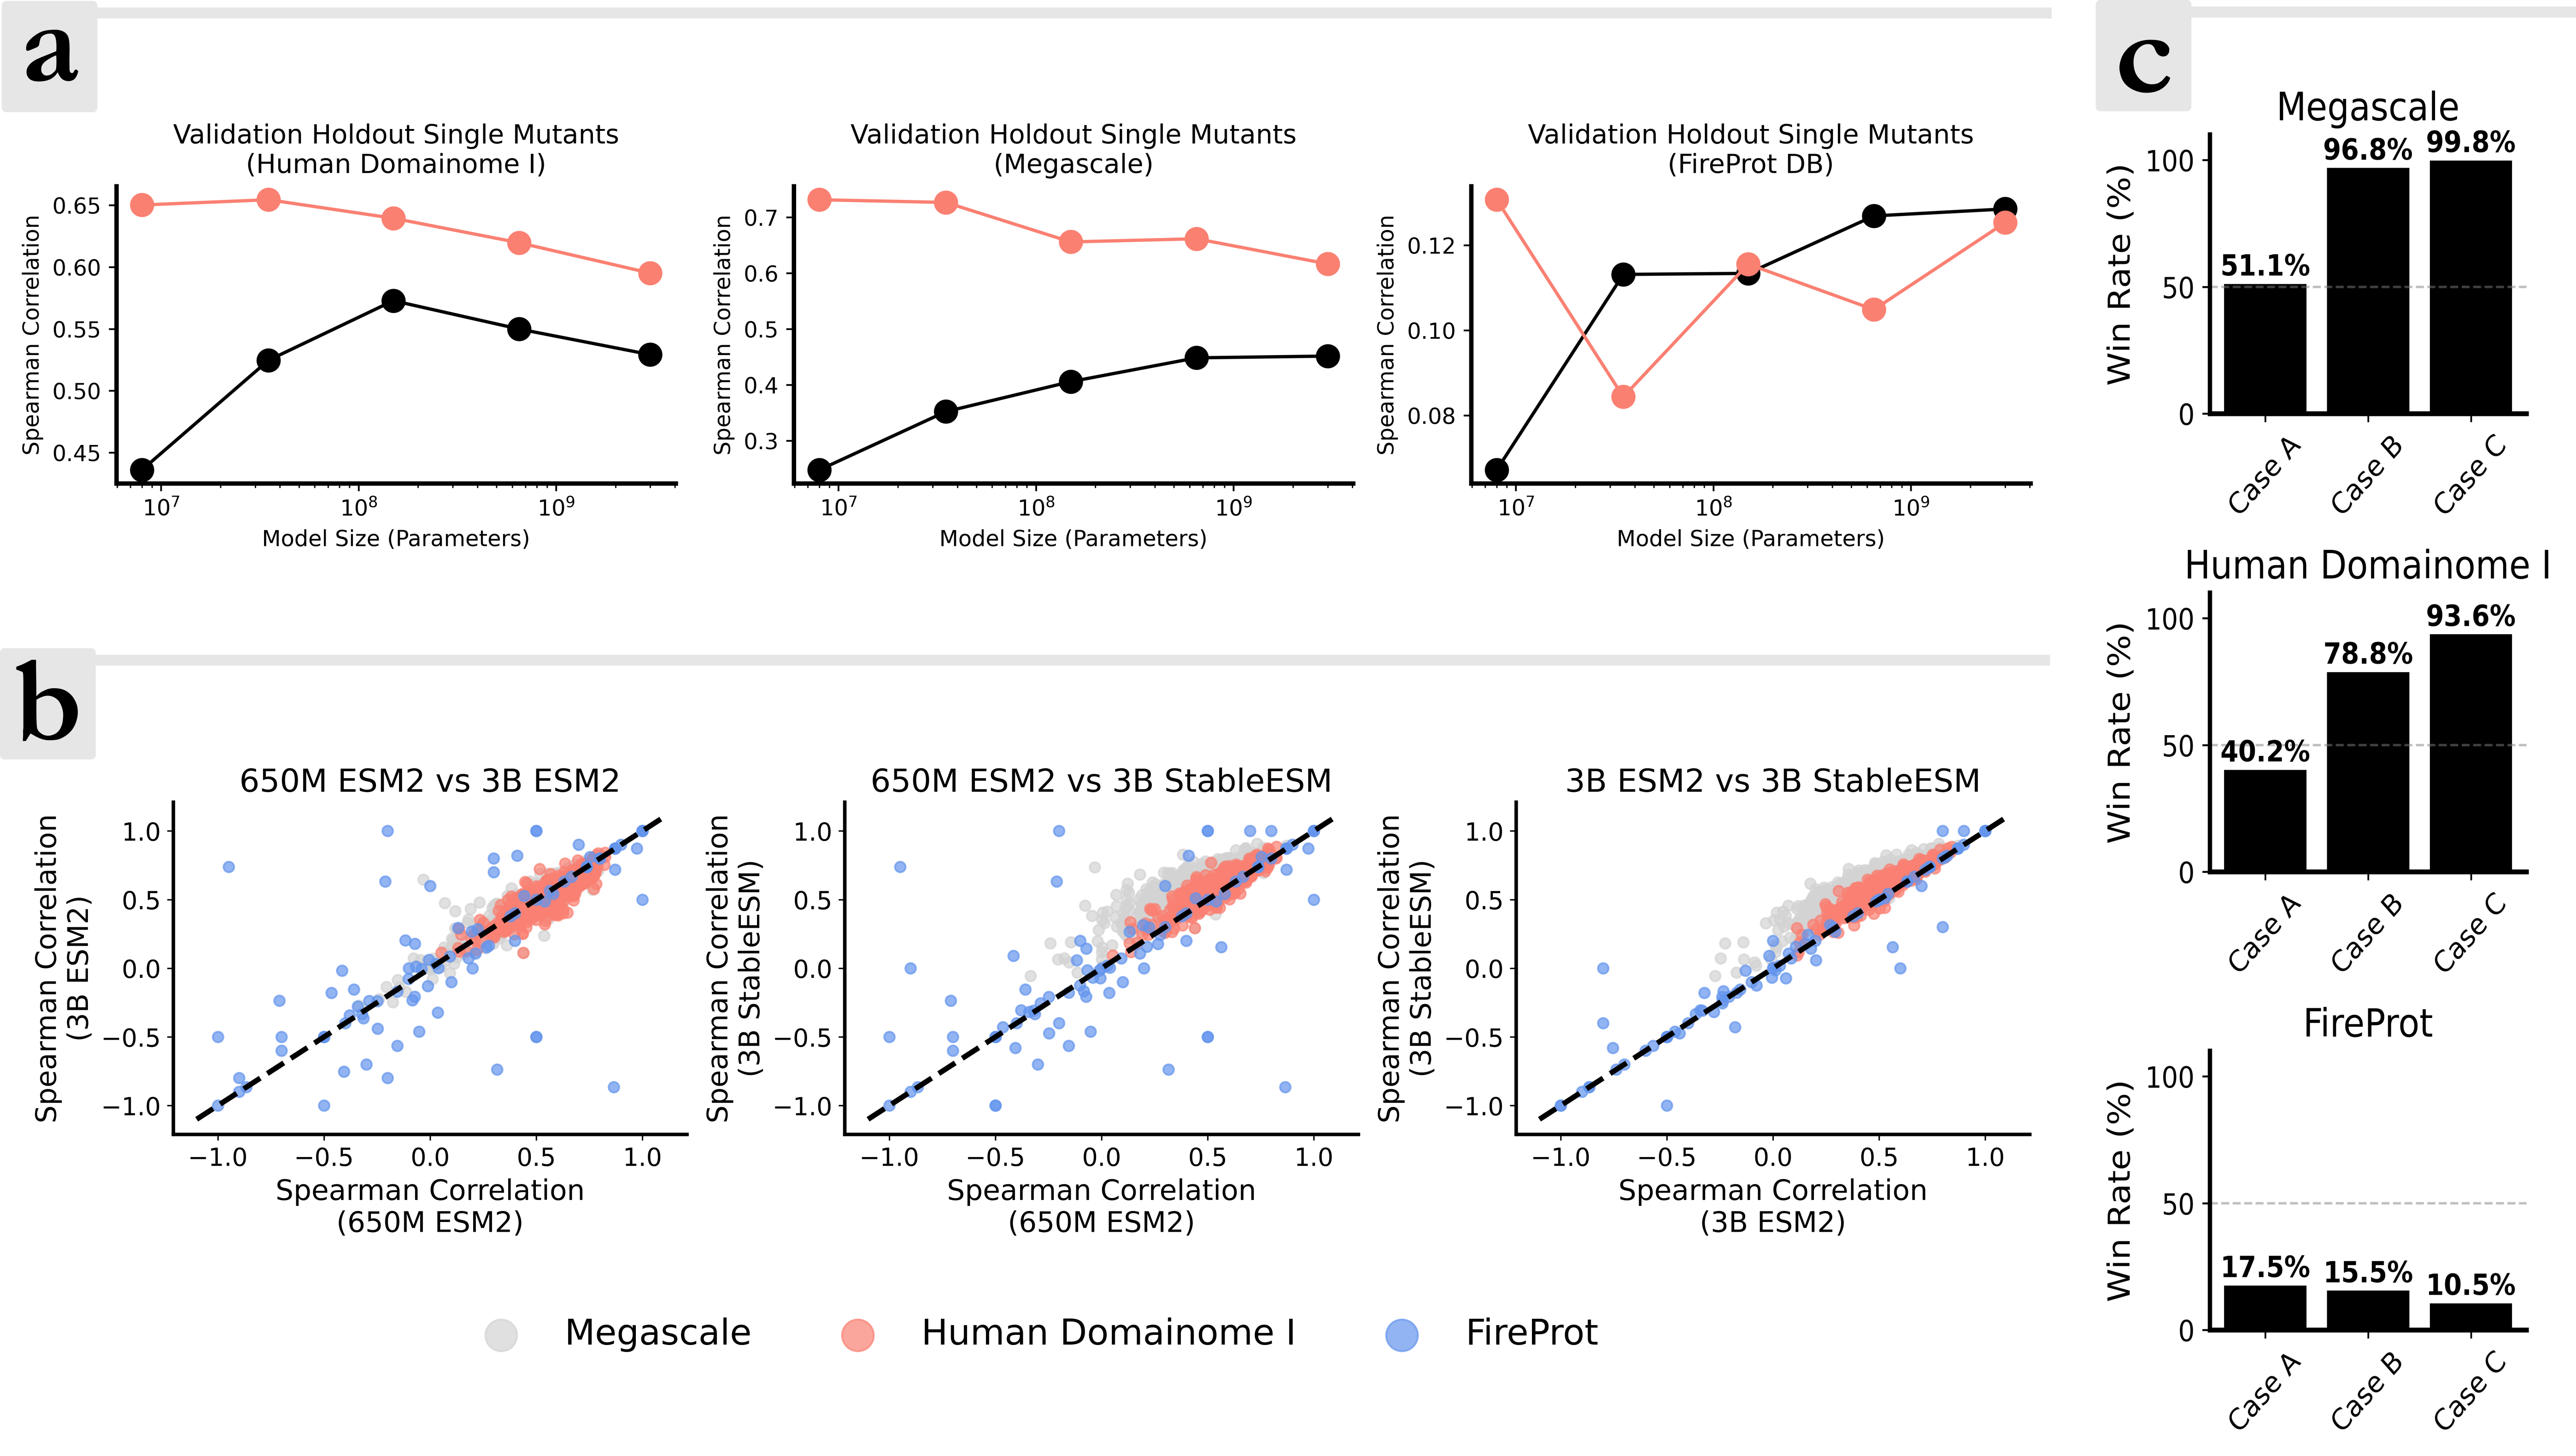
\includegraphics[width=1.0\linewidth]{figures/extended_figures/Figure_Extended_2.png}
    \caption{\textbf{StableESM demonstrates consistent validation performance improvements across datasets and model scales.} \textbf{(a)} Per-domain Spearman correlations on validation single mutants held out during training. StableESM (red) consistently outperforms ESM2 (black) across all model sizes on MegaScale and Human Domainome I datasets, with StableESM 3B achieving superior performance compared to ESM2 650M, consistent with literature reports that ESM2 3B saturates in performance against ESM2 650M while StableESM breaks this scaling limitation. FireProt shows minimal improvement, likely due to limited mutation quantity in this dataset. \textbf{(b)} Pairwise model comparisons on per-domain correlations. While scaling from ESM2 650M to 3B shows no improvement (Case A), StableESM 3B demonstrates clear superiority over both ESM2 650M (Case B) and ESM2 3B (Case C) on MegaScale and Human Domainome I datasets, with most domains falling above the diagonal. \textbf{(c)} Win-rate analysis quantifying the fraction of domains where one model outperforms another. ESM2 3B performs comparably or worse than ESM2 650M across datasets (Case A), while StableESM 3B achieves dramatic win-rates of 96.8\% and 78.8\% against ESM2 650M (Case B) and 99.8\% and 93.6\% against ESM2 3B (Case C) on MegaScale and Human Domainome I, respectively, demonstrating that preference alignment unlocks the scaling potential of larger protein language models.}
    \label{fig: eval_on_valid_holdout}
\end{figure}  

\begin{figure}[h!]
    \centering
    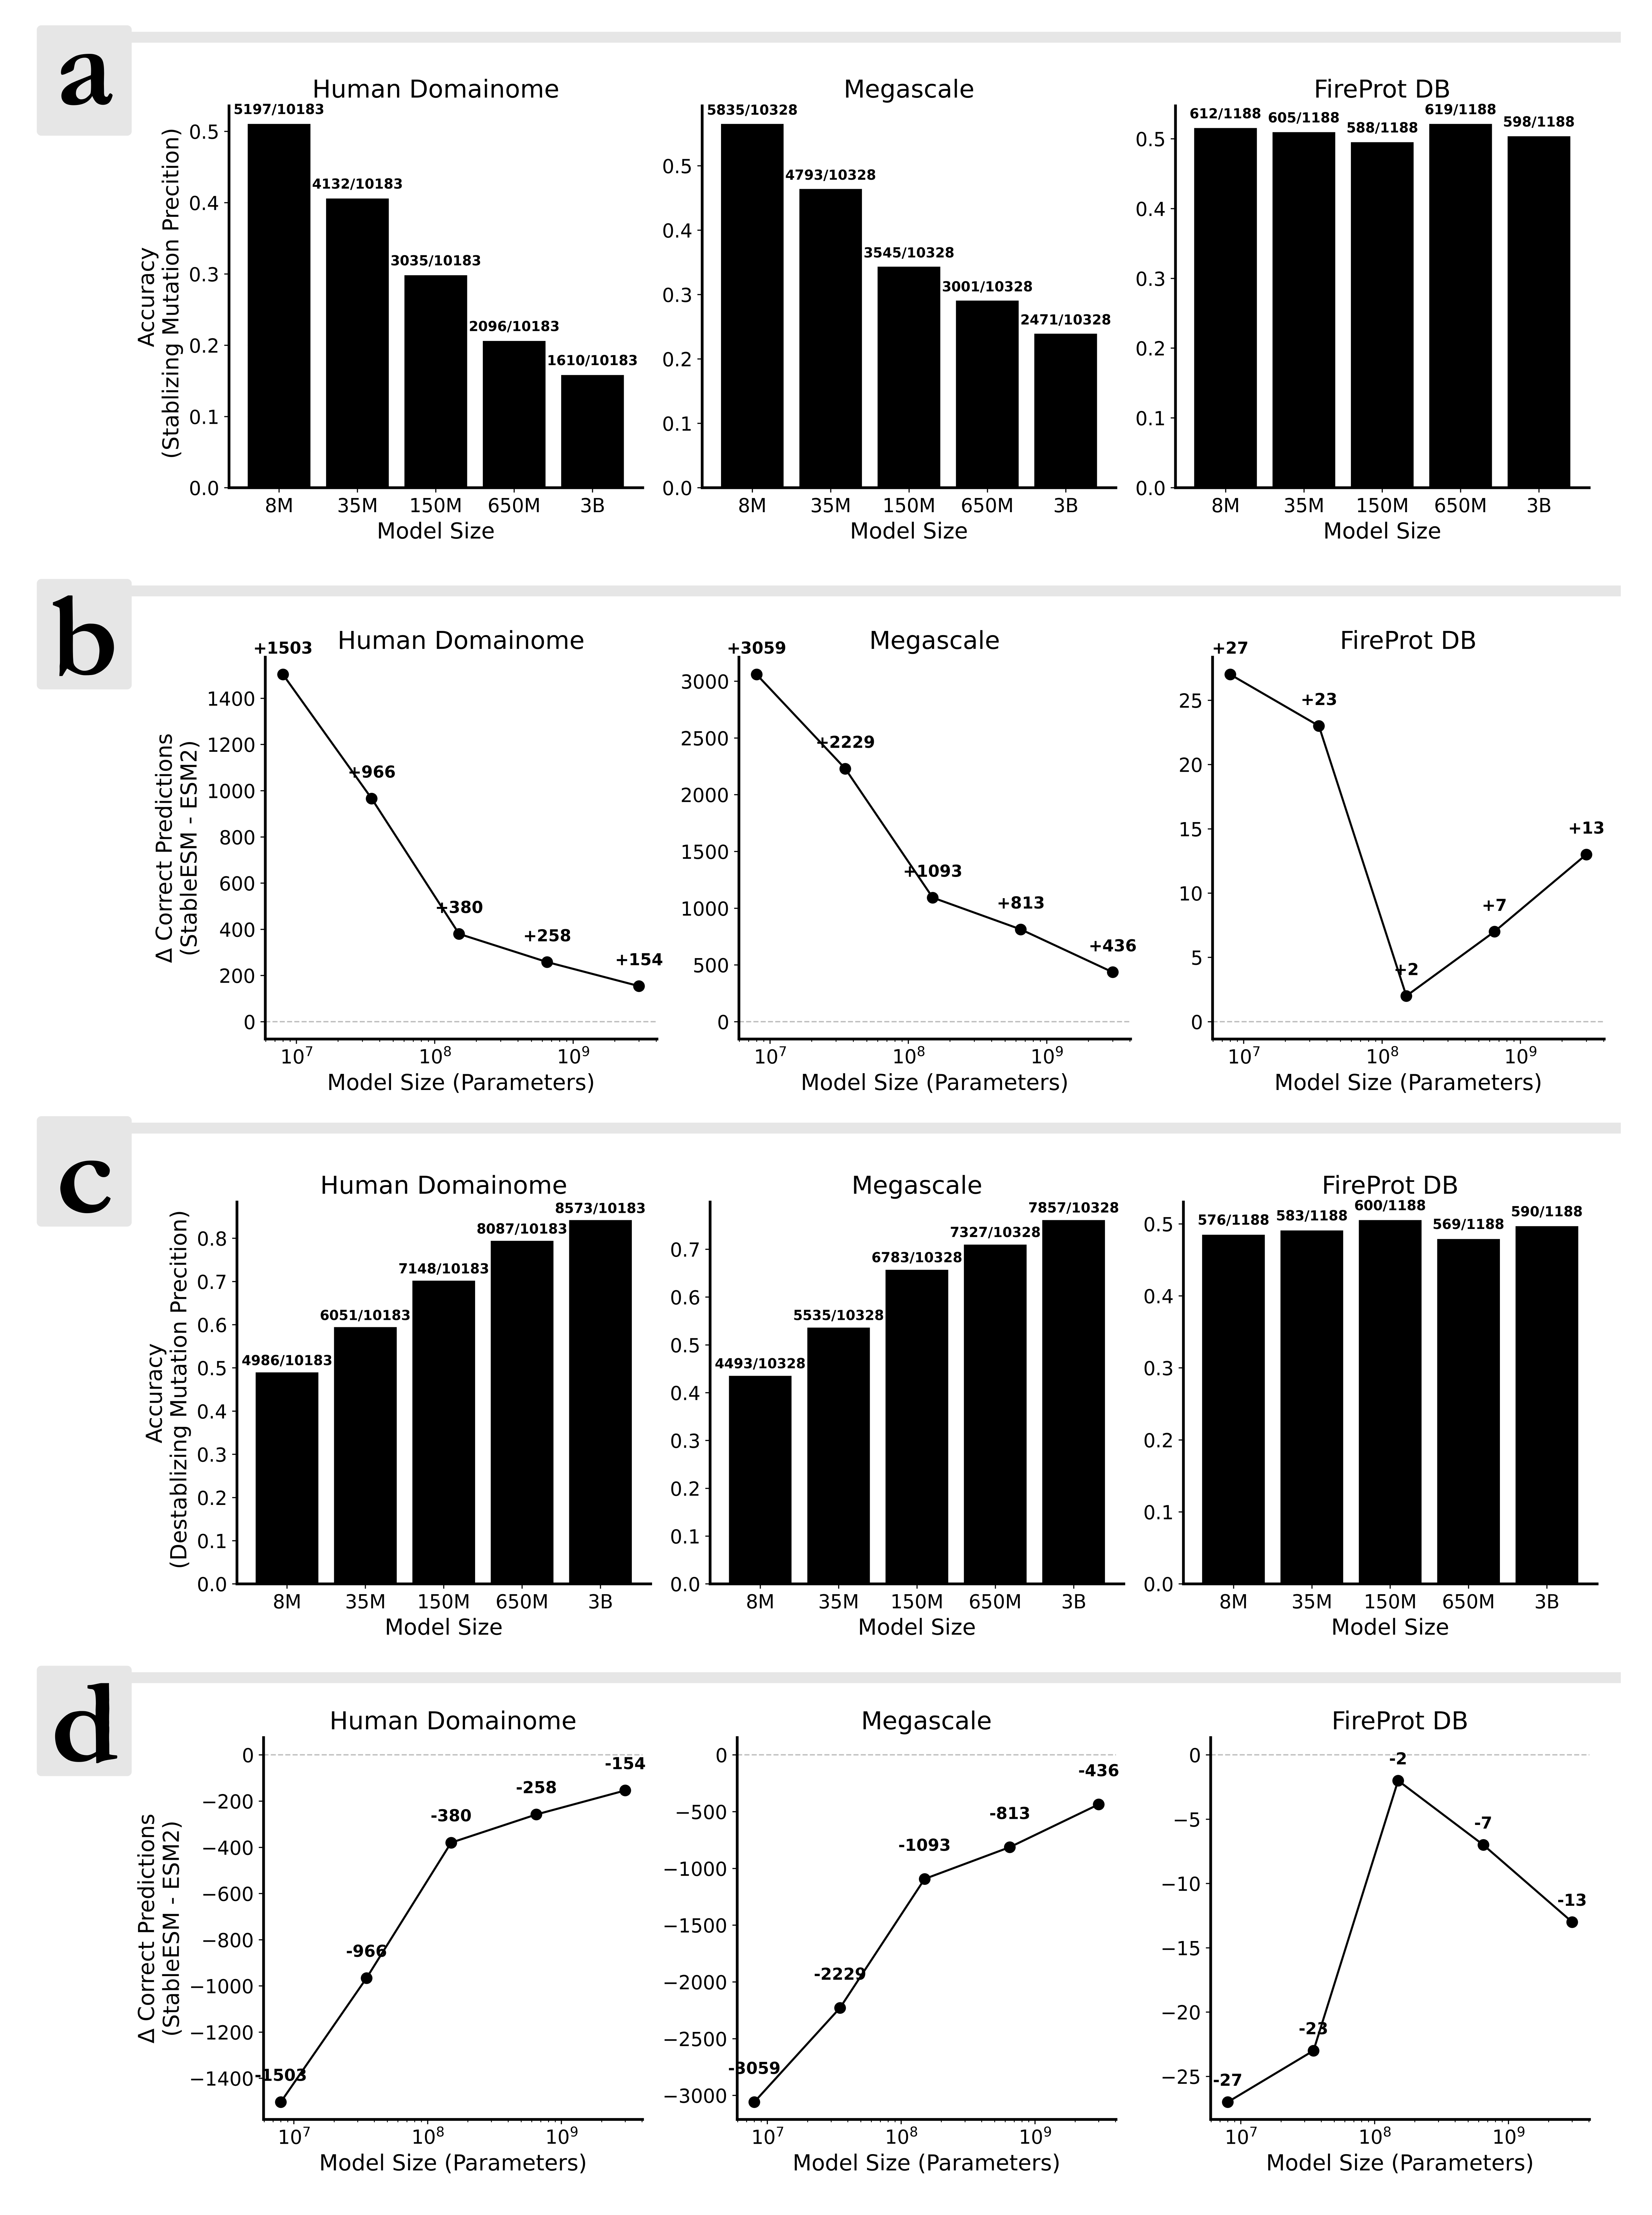
\includegraphics[width=1.0\linewidth]{figures/extended_figures/Figure_Extended_3.png}
    %\caption{}
    %\label{fig: eval_classification_on_valid_holdout}
\end{figure}



\captionof{figure}{\textbf{StableESM improves classification of both stabilizing and destabilizing mutations across model scales on validation holdout mutants, addressing known limitations in gain-of-function prediction.} \textbf{(a)} Accuracy for predicting stabilizing mutations (gain-of-function) on validation holdout mutants not seen during training. StableESM demonstrates improved performance across all model sizes on Human Domainome and Megascale datasets, with larger models achieving higher accuracy. FireProt DB shows consistently high performance across scales due to dataset characteristics. Numbers above bars indicate correct predictions over total stabilizing mutations. \textbf{(b)} Improvement in correct stabilizing mutation predictions (StableESM - ESM2) on validation holdout sets. All StableESM models show substantial gains over ESM2 baselines, with larger models being able to achieve improvements (+154, +436, +13 additional correct predictions for Human Domainome, Megascale, and FireProt DB respectively at 3B scale). \textbf{(c)} Accuracy for predicting destabilizing mutations on validation holdout mutants, where larger protein language models traditionally excel. StableESM maintains strong performance across scales while showing the expected scaling behavior where larger models achieve higher accuracy ($\sim$2x improvement from 8M to 3B), consistent with literature. \textbf{(d)} Improvement in correct destabilizing mutation predictions (StableESM - ESM2) on validation holdout sets. While larger StableESM models show modest improvements over ESM2 for deleterious predictions, smaller models like 8M exhibit high false positive predictions. These results demonstrate that larger StableESM models effectively address the known limitation of protein language models in gain-of-function prediction while preserving their established strength in identifying deleterious mutations~\citep{ertelt2025self}, suggesting that preference alignment at scale unlocks balanced performance across both stabilizing and destabilizing mutation classes.}
\label{fig: eval_classification_on_valid_holdout}


\begin{figure}[h!]
    \centering
    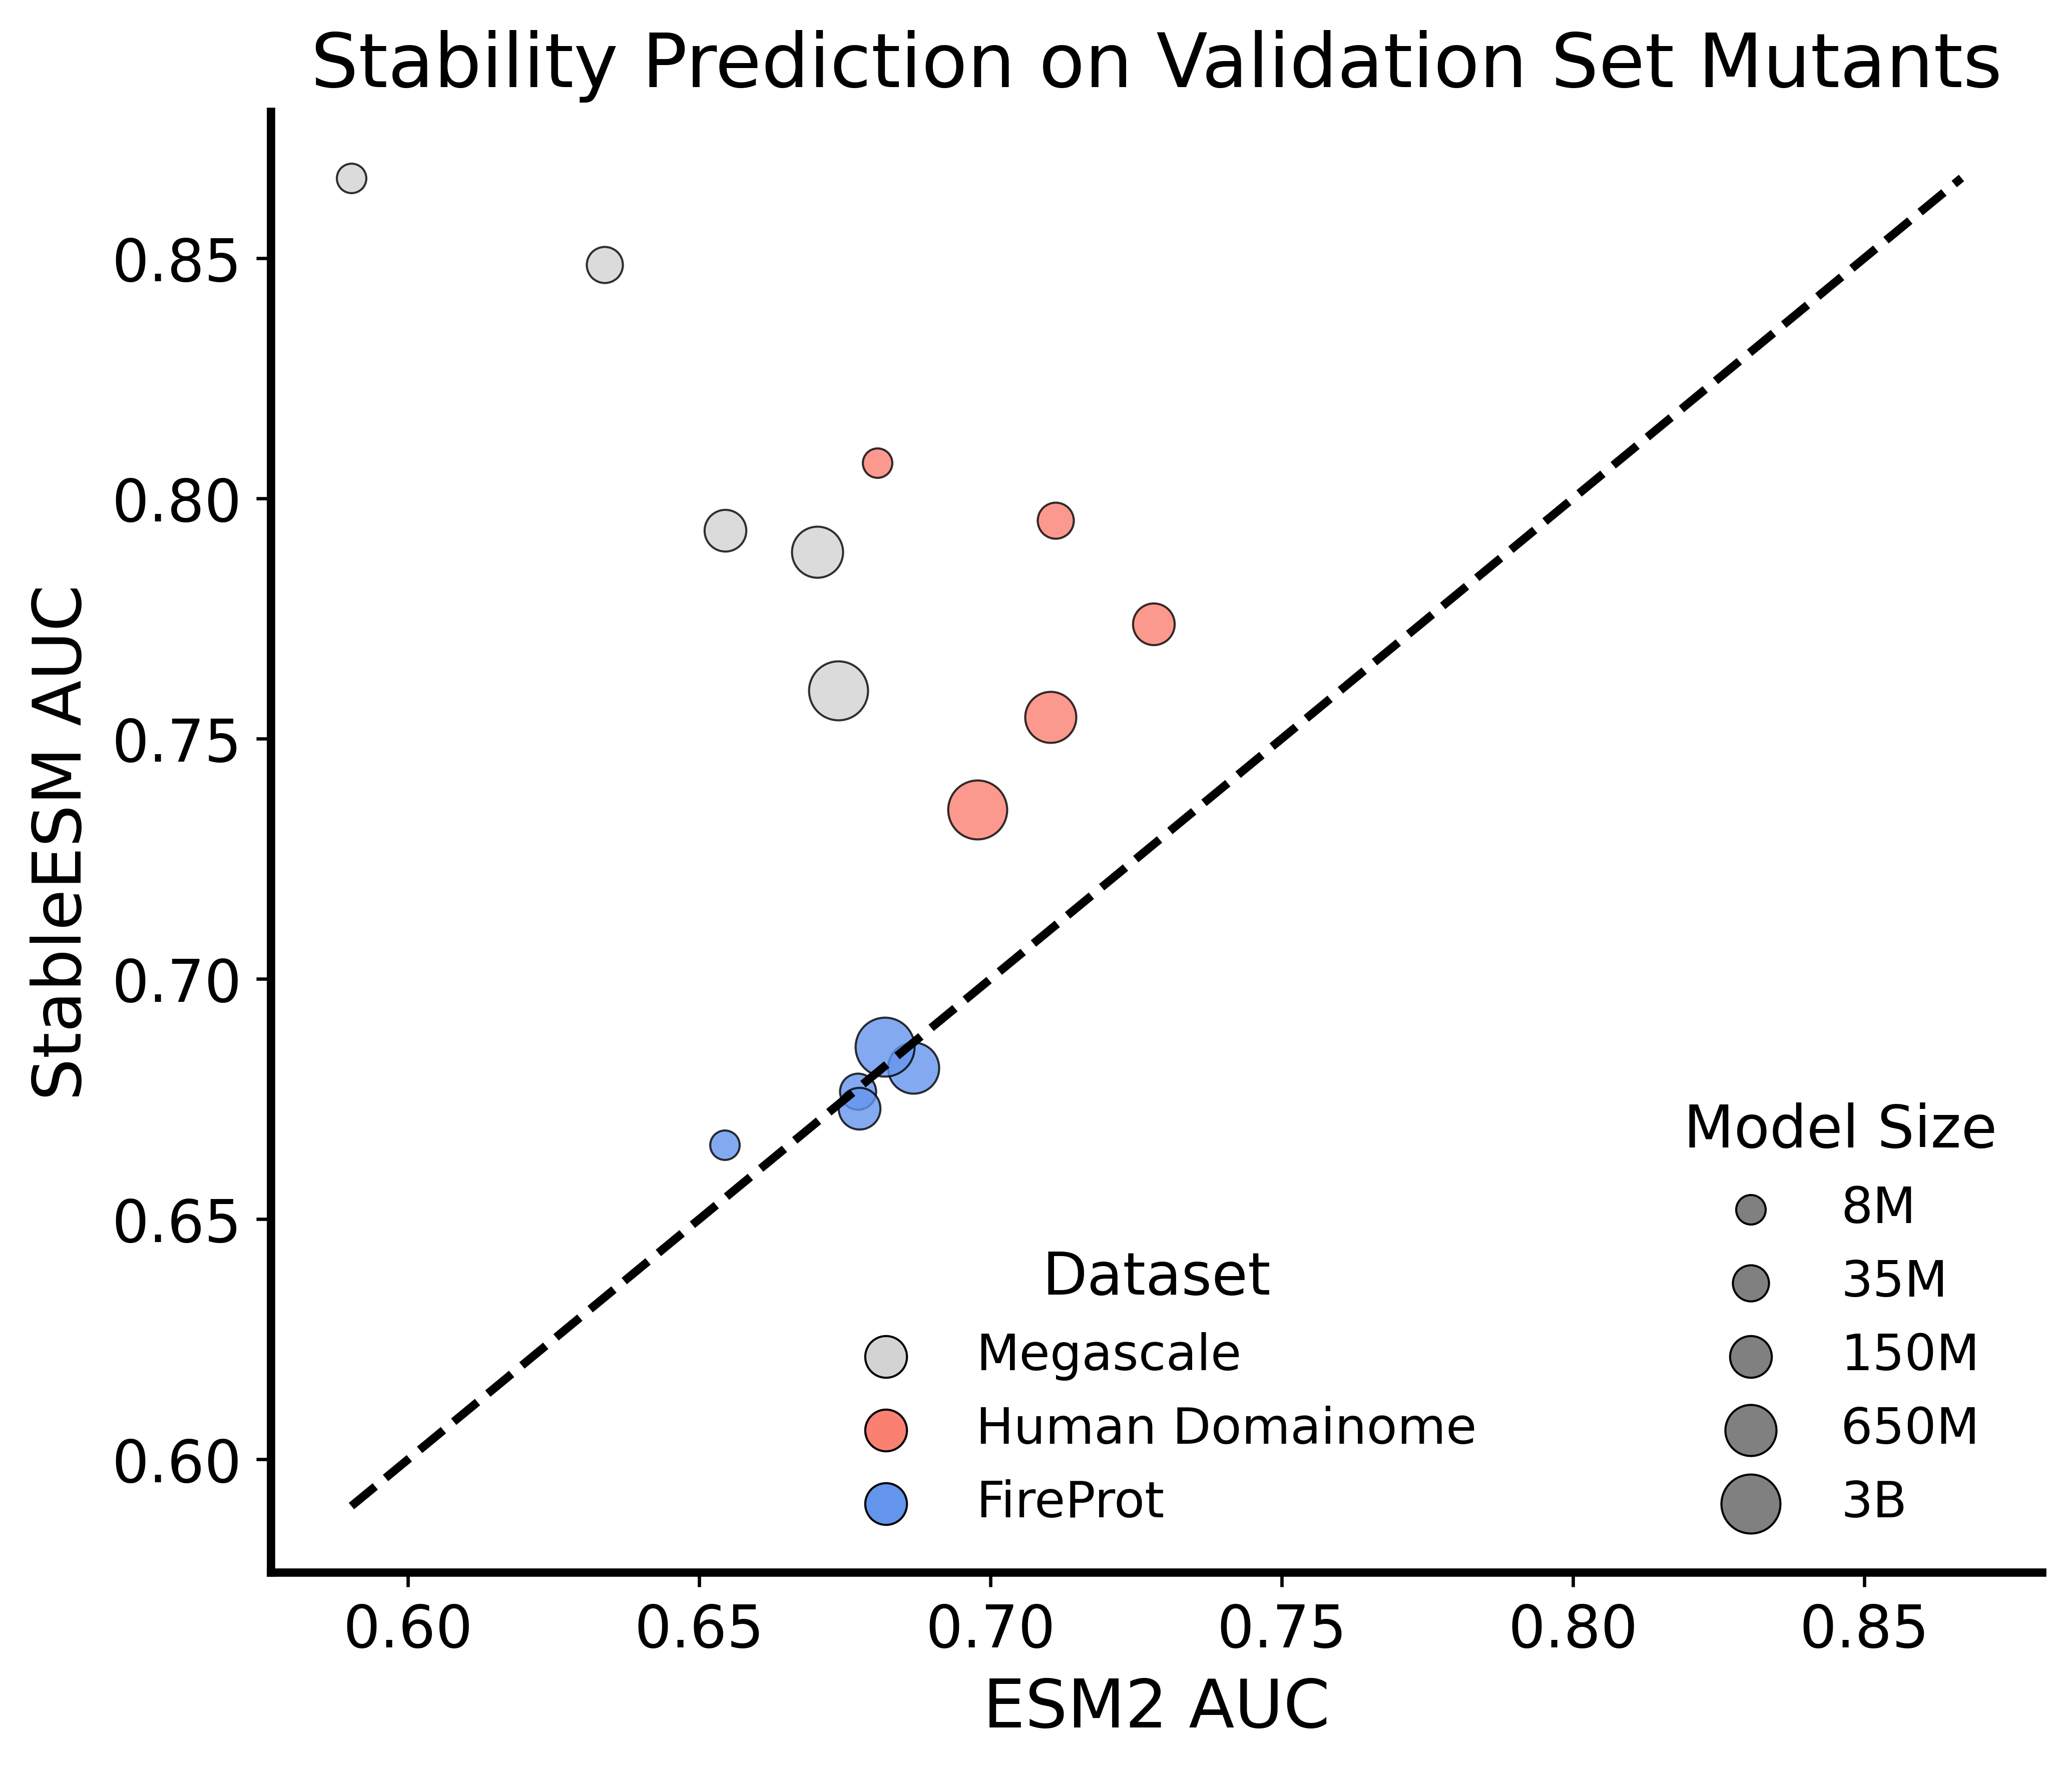
\includegraphics[width=0.6\linewidth]{figures/extended_figures/Figure_Extended4.png}
    \caption{\textbf{StableESM consistently outperforms ESM2 across all model sizes and datasets for stability prediction on validation holdout single mutants.} Each point represents AUC scores for classification of stabilizing versus destabilizing mutations, with ESM2 performance on the x-axis and StableESM performance on the y-axis. Point colors indicate dataset (grey: Megascale, red: Human Domainome, blue: FireProt) and sizes represent model scale (8M to 3B parameters). All points fall above the diagonal line, demonstrating that StableESM achieves superior classification performance compared to ESM2 across all tested conditions. Human Domainome and Megascale datasets show substantial improvements, while FireProt exhibits more modest but consistent gains. The results demonstrate that preference alignment provides robust benefits for mutation effect classification regardless of model size or dataset characteristics, with improvements ranging from  $\sim$0.01 to $\sim$0.08 AUC units across the tested conditions.}
    \label{fig: auc_comparison_val_holdout}
\end{figure}



\begin{figure}[h!]
    \centering
    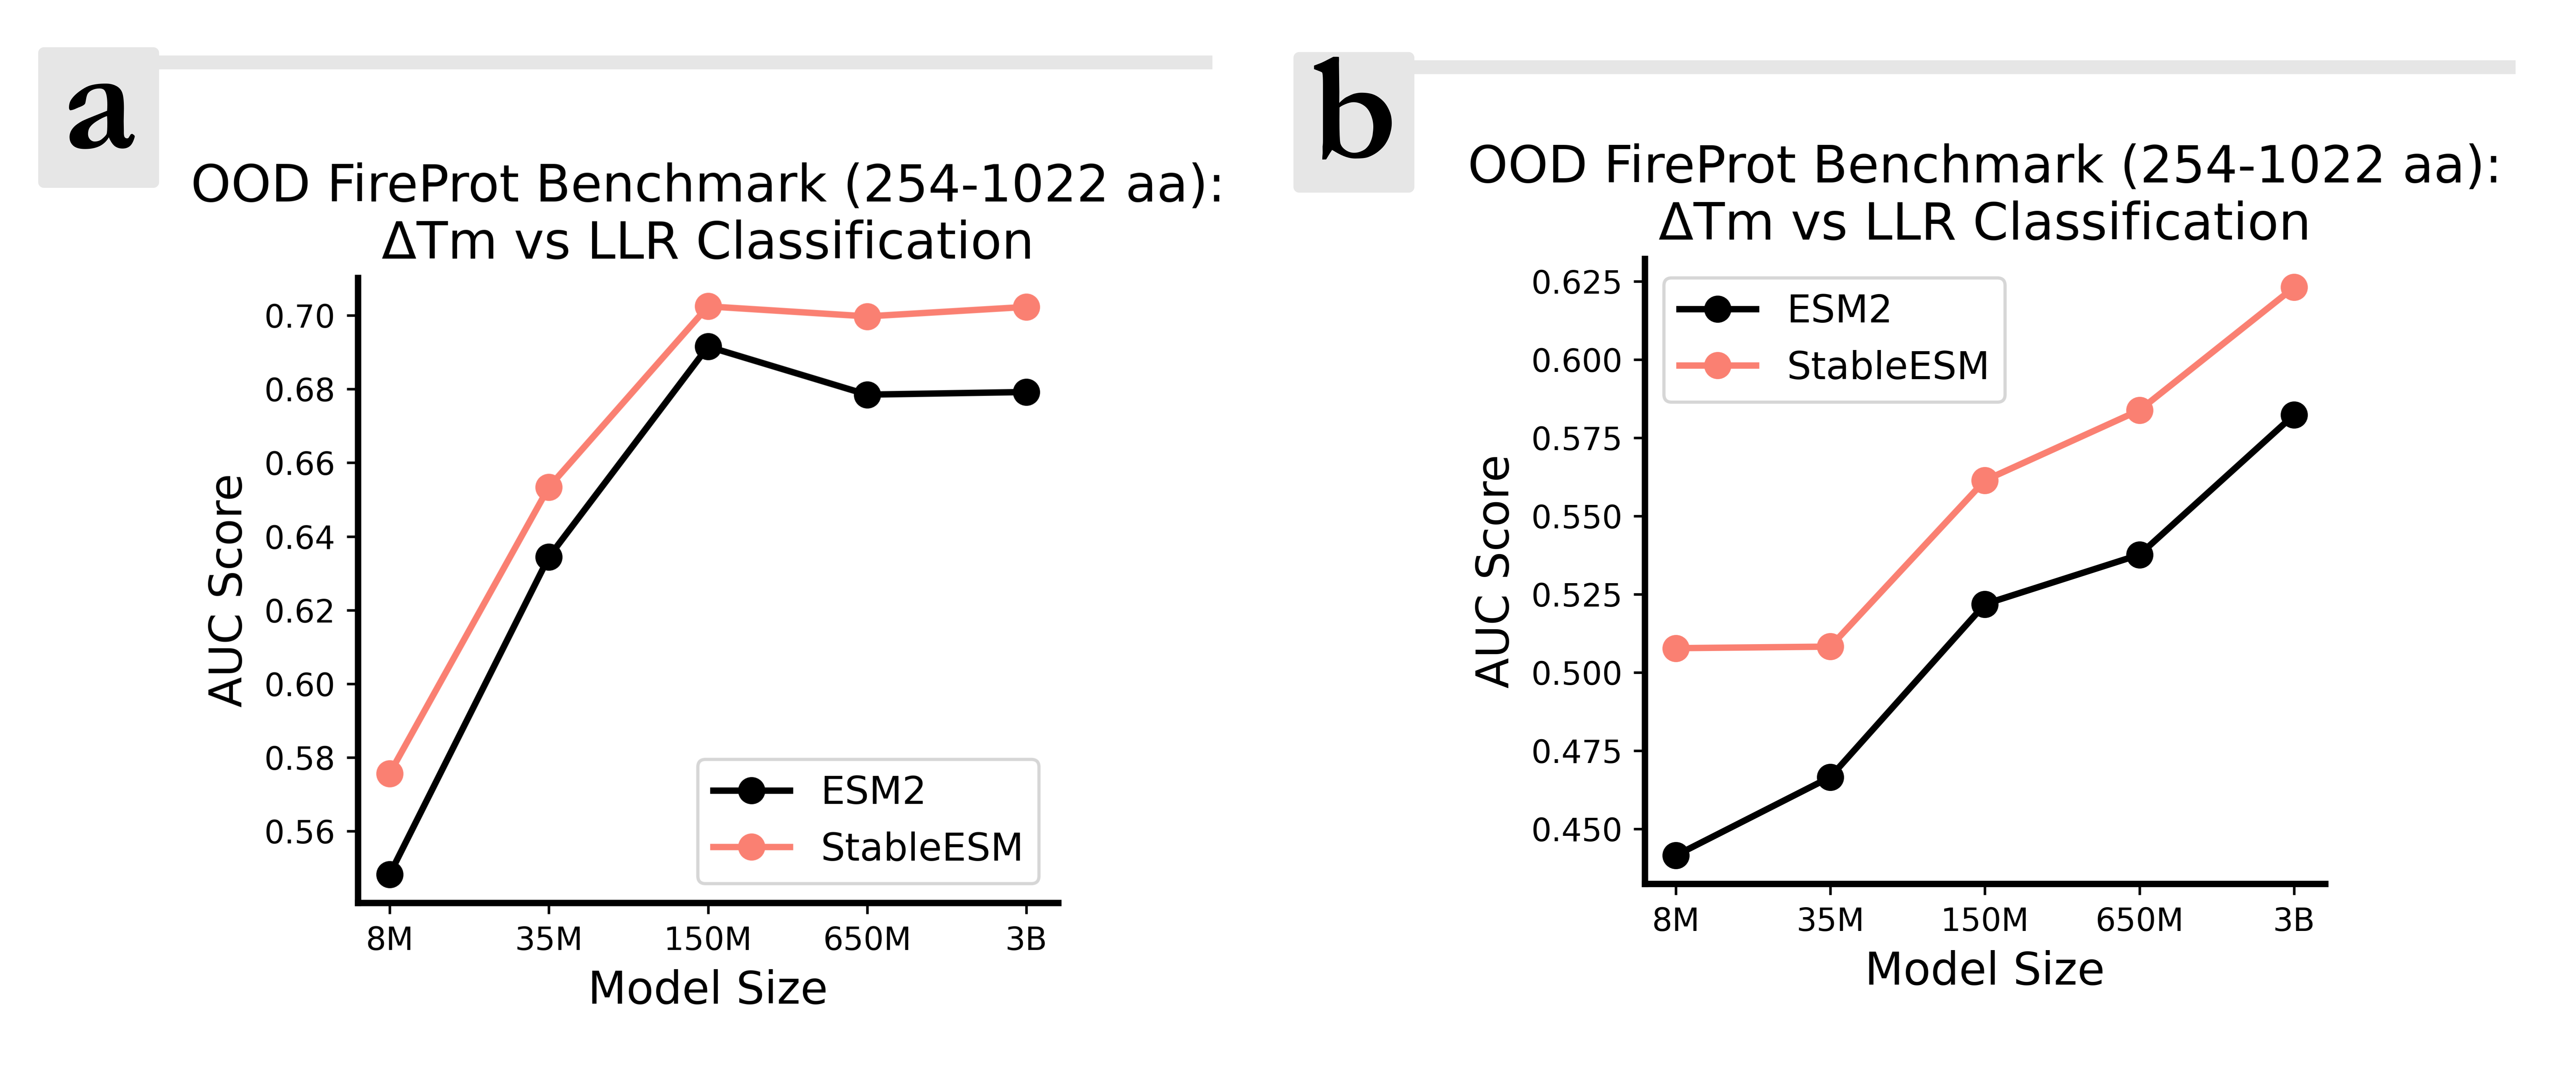
\includegraphics[width=1.0\linewidth]{figures/extended_figures/Figure_Extended5.png}
    \caption{\textbf{StableESM demonstrates improved classification performance on out-of-distribution (OOD) FireProt benchmark proteins (254-1022 amino acids).} \textbf{(a,b)} Area under the curve (AUC) scores for classifying stabilizing versus destabilizing mutations using $\Delta T_m$ measurements on completely held-out protein domains. StableESM (red) consistently outperforms ESM2 (black) across all model sizes, with performance improvements ranging from  $\sim$0.01 AUC units at smaller scales to  $\sim$0.05 AUC units at 3B parameters. While ESM2 performance plateaus at larger model sizes, StableESM continues to benefit from increased scale, achieving AUC scores of 0.71 and 0.625, respectively. These results complement the Spearman correlation analysis in Figure~\ref{fig:train_eval_stableesm}e, demonstrating that preference alignment not only improves zero-shot mutant effect prediction performance but also enhances binary classification of mutation effects on out-of-distribution protein domains, suggesting that preference alignment improves on better classifying gain-of-stability and deleterious effects.}
    \label{fig: eval_classification_on_valid_holdout}
\end{figure}


\begin{figure}[h!]
    \centering
    \includegraphics[width=1.0\linewidth]{figures/extended_figures/Figure_Extended6_final.png}
    \caption{\textbf{Preference alignment enables StableESM to generalize to out-of-distribution protein domains with improved mutational effect prediction.} \textbf{(a)} Distribution of Spearman correlation improvements (StableESM - ESM2) at 3B parameters for FireProtDB protein domains (224-1022 amino acids,$\geq$30 mutations per domain). StableESM significantly outperforms ESM2 on this out-of-distribution set (Wilcoxon signed-rank test: W = 145, p = 0.000191), with 94\% of domains showing improved rank correlation.\textbf{(b)} Model scaling analysis for the domain with largest improvement: Tyrosine-protein kinase Fyn (UniProt: P06241, 537 amino acids). StableESM 3B achieves exceptional correlation ($\rho$ = 0.886) compared to ESM2 models across all scales, demonstrating that preference alignment on shorter sequences ($\leq$224 amino acids during training) generalizes to substantially longer, unseen proteins. \textbf{(b)} Experimental validation showing relationship between $\Delta T_m$ measurements and StableESM 3B log-likelihood ratios for Tyrosine-protein kinase Fyn, with AlphaFold structure representation (grey). These results demonstrate that preference alignment enables robust generalization beyond the length distribution encountered during training, achieving strong predictive performance on completely out-of-distribution protein domains.}
    \label{fig: generalize_OOD_fireprot_StableESM}
\end{figure}


\begin{figure}[h!]
    \centering
    \includegraphics[width=1.0\linewidth]{figures/extended_figures/Figure_Extended7_final.png}
 \caption{\textbf{Preference alignment of StableESM improves binary classification of mutational effects on out-of-distribution set.} \textbf{(a)} AUC difference between StableESM and ESM2 at 3B parameters for protein domains with lengths between 224 and 1022 amino acids from the FireProtDB dataset. Only domains with $\geq$30 mutations were included to ensure robust AUC calculations. A Wilcoxon signed-rank test confirmed that StableESM significantly improves binary classification performance on the out-of-distribution (OOD) set (p $<$ 0.001). Additionally, 64.7\% of domains showed improved AUC scores. \textbf{(b)} Analysis of the domain with substantial improvement: Polyubiquitin (UniProt: P0CG63), which showed an AUC difference of 0.128 for the 3B model. This protein has a length of 381 amino acids, substantially longer than any sequence seen during preference alignment (maximum 224 amino acids), demonstrating that preference alignment on a large corpus of stability mutations can generalize to longer, unseen proteins. The progression from ESM2 (8M) at 0.333 AUC to StableESM (3B) at 0.609 AUC illustrates consistent improvement with model scale and alignment. \textbf{(c)} Relationship between experimental $\Delta\Delta G$ values and log-likelihood ratio scores from StableESM (3B) for Polyubiquitin, with AlphaFold structure representation (grey). A cubic polynomial fit (red line, $R^2$ = 0.2160) shows the model's ability to distinguish between stabilizing (negative $\Delta\Delta G$) and destabilizing (positive $\Delta\Delta G$) mutations, with the downward arrow ($\downarrow$) indicating that negative $\Delta\Delta G$ values correspond to increased protein stability.}
    \label{fig: generalize_auc_OOD_fireprot_StableESM}
\end{figure}



